%This is not for dummies, but for mere m0rtals
%%This is a very basic article template.
%%There is just one section and two subsections.
%\documentclass{article}
\documentclass[a4paper,11pt]{article}
%\documentclass[letterpaper,11pt]{article}

\usepackage{url}
\usepackage{hyperref}
\usepackage{breakurl}

\usepackage{multicol}
%\usepackage{times}
\usepackage{charter}    % Charter
\usepackage{courier}    % Courier, \texttt only
\usepackage{float}      % floating graphics 
\usepackage{graphicx}
\usepackage{wrapfig}
%\usepackage{hyperref}
\usepackage{listings}
\hypersetup{colorlinks=false}
\hypersetup{
    colorlinks,%
    citecolor=black,%
    filecolor=black,%
    linkcolor=black,%
    urlcolor=black,%
    breaklinks=true,%
}

% Quite good monospace-font:
\renewcommand{\ttdefault}{txtt}


% box for Verbatim
\usepackage{verbatim}
\usepackage{framed}


\usepackage[top=2cm, bottom=2cm, left=2cm, right=2cm]{geometry} 
\usepackage{sectsty}
\sectionfont{\Large}

\lstset{
numbers=left, 
stepnumber=1, 
frame=single, 
breaklines=true,
breakatwhitespace=false, 
frame=shadowbox, 
rulesepcolor=\color{black},
basicstyle = \ttfamily,
columns=fullflexible
}

\long\def\greybox#1{%
    \newbox\contentbox%
    \newbox\bkgdbox%
    \setbox\contentbox\hbox to \hsize{%
        \vtop{
            \kern\columnsep
            \hbox to \hsize{%
                \kern\columnsep%
                \advance\hsize by -2\columnsep%
                \setlength{\textwidth}{\hsize}%
                \vbox{
                    \parskip=\baselineskip
                    \parindent=0bp
                    #1
                }%
                \kern\columnsep%
            }%
            \kern\columnsep%
        }%
    }%
    \setbox\bkgdbox\vbox{
        \pdfliteral{0.85 0.85 0.85 rg}
        \hrule width  \wd\contentbox %
               height \ht\contentbox %
               depth  \dp\contentbox
        \pdfliteral{0 0 0 rg}
    }%
    \wd\bkgdbox=0bp%
    \vbox{\hbox to \hsize{\box\bkgdbox\box\contentbox}}%
    \vskip\baselineskip%
}

%\newcommand{\ScriptsDir}{../../../../eldk-5-0-scripts}
%\newcommand{\DenxDir}{../../../../eldk-5-0-denx}

\begin{document}
\thispagestyle{empty} % no page number

\begin{figure}
 \begin{center}
  
\includegraphics[width=0.35\textwidth]{res-logo-mirror}
 \end{center}
\end{figure}

\begin{center}
\section*{FreeRTOS on PIC 18 for mere m0rtals}
Robert Berger - Reliable Embedded Systems - Consulting Training Engineering \\http://www.ReliableEmbeddedSystems.com\\ robert.berger@ReliableEmbeddedSystems.com
\end{center}

\section{Disclaimer}
The views, opinions, positions or strategies expressed by the author and those
providing comments are theirs alone, and do not necessarily reflect the views,
opinions, positions or strategies of anybody else.

\section{Acknowledgements}
Many thanks go to Isaac Marino Bavaresco~\cite{isaac-site}~\cite{piclist-site}
and Richard Barry~\cite{freertos-site} for their continuous support.

\section{FAQ for this document}
\subsection{Hyper-links}
Please note, that within the pdf file hyper-links (cursor changes shape when you
move it over a hyper-link) should be working most of the time. Just click on them
and give it a try. Sometimes they are broken into multiple lines and you might
need to fiddle around with them a bit.
% \subsection{Where to put the scripts?}
% Please refer to the section~\ref{sec:dirstruct} where you can see a
% tree-like outline of the directory structure which works for me.

\section{Introduction}
We'll have a look at porting FreeRTOS~\cite{freertos-site} to a
micro-controller from Microchip's~\cite{microchip-site} PIC18 family. Many
people will say that's impossible/difficult/overkill and exactly that's the
reason why I'm trying to show how it can be done.

\section{Hardware}
Tests were performed with a the PIC18 Explorer + PIC18LF45K22 PIM (switch S4
needs to be in position ICE to choose the PIM over the chip, which is soldered
on the PIC18 Explorer board) and a REAL ICE in circuit emulator.
 \begin{center}
  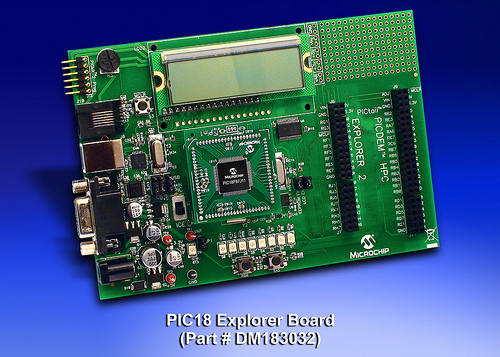
\includegraphics[width=0.35\textwidth]{PIC18-Explorer-board}
 \end{center}

 \begin{center}
  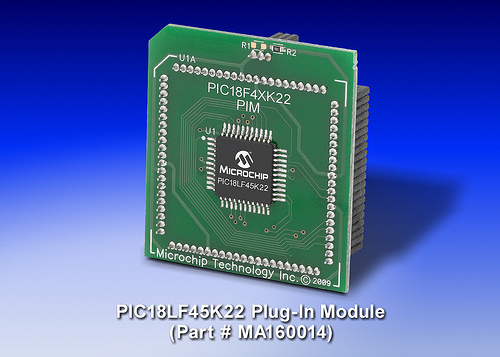
\includegraphics[width=0.35\textwidth]{PIC18LF45K22-PIM}
 \end{center}

 \begin{center}
  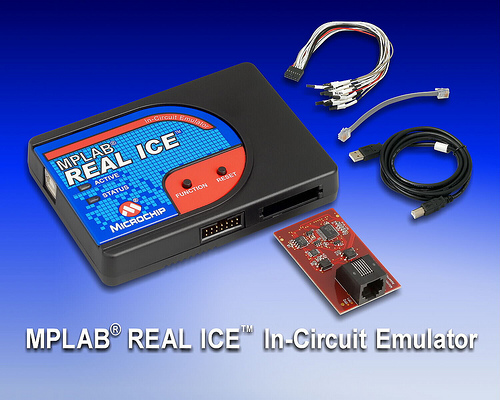
\includegraphics[width=0.35\textwidth]{Real-ICE}
 \end{center}

 \begin{center}
  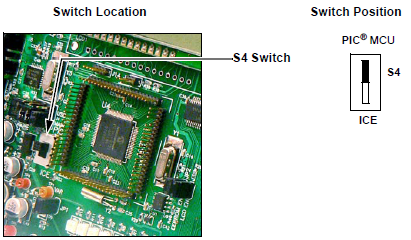
\includegraphics[width=0.35\textwidth]{board-S4}
 \end{center}

\section{Toolchain}
At the time of writing the latest and greatest MPLAB IDE and C18 were MPLAB
IDE v8.73 and MPLABC18 v3.39.

\section{Getting started}
\emph{You don't need to follow those instruction, since I made something much
easier (see below) which you might want to use.} 

\subsection{FreeRTOS V5.3.0 for 18f2620}

I followed the instructions on solar-blog~\cite{solar-blog-site} and got some
old version of FreeRTOS compiled with goodies from Isaac and for the PIC18f2620
instead of the the PIC18LF45K22.

You can get a MPLAB project here:
\lstinputlisting{freertos-18f2620-original-zip.txt}

Just copy it to C:/projects/microchip/\ldots and it should be an ''out of the
box'' experience. 

Let's have a look at some of the goodies, which come form Isaac. 

\subsubsection{Heap management for small microcontrollers~\cite{isaac-heap}}
The PIC18 has a (banked) memory architecture and also typically a very small
amount of RAM which makes it badly suited for Real Time operating systems. This
library is specially suited for PIC18 with FreeRTOS and Microchip MPLAB-C18.

\begin{itemize}
  \item optimized {\tt malloc()}, {\tt free()}
  \item Heap and Stack should be joined together
  \item {\tt \_\_reclaim\_stack()}    
\end{itemize}

\subsubsection{MATH\_DATA \& .tmp\_data save/restore for
FreeRTOS~\cite{isaac-math}}
The ''official'' port of FreeRTOS for PIC18 with Microchip MPLAB-C18 has some
problems when saving and restoring the compiler-generated memory sections
"{\tt MATH\_DATA}" and "{\tt .tmpdata}" and newer C18 compilers. This solution
appears to be version-independent.


\subsection{FreeRTOS V5.3.0 for PIC18LF45K22}
For the above to work on the PIC18LF45K22 we need to adjust a few things.
\subsubsection{Linker script}
Note that small sections are joined together to form a bigger section.
\lstinputlisting{linker-script.diff}
\subsubsection{configuration for heap library}
Note that we should tell the heap library that the stack is after the heap with
\lstinputlisting{heap-config.txt}
\lstset{language=c}
\lstinputlisting{heap-config.diff}
{\tt not much changed in here, have a look at {\tt static void
prvSetupTimerInterrupt (void)}}
\lstinputlisting{port-c.diff}

\subsection{FreeRTOS V7.0.1 for PIC18LF45K22}
Theoretically we just need a bit for copying/merging;)

\pagebreak

\begin{thebibliography}{}

  \bibitem{freertos-site} \textsl{''FreeRTOS''}
  \url{http://www.freertos.org/}

  \bibitem{microchip-site} \textsl{''Microchip''}
  \url{http://www.microchip.com/}

  \bibitem{isaac-site} \textsl{''Homepage for Isaac Marino Bavaresco''}
  \url{http://www.sxlist.com/techref/member/IMB-yahoo-J86/index.htm}
  
  \bibitem{isaac-heap} \textsl{''Heap management for small microcontrollers''}
  \url{http://www.sxlist.com/TECHREF/member/IMB-yahoo-J86/heap-mgmt.htm}
  
  \bibitem{isaac-math} \textsl{''MATH\_DATA \& .tmp\_data save/restore for
  FreeRTOS''}
  \url{http://www.sxlist.com/TECHREF/member/IMB-yahoo-J86/math_data_tmp_data.htm}

  \bibitem{solar-blog-site} \textsl{''Setting Up FreeRTOS for the PIC18 Using MPLAB C18''}
  \url{http://solar-blogg.blogspot.com/search/label/PIC18}

  \bibitem{piclist-site} \textsl{''Piclist''} 
  \url{http://www.piclist.com/}

\end{thebibliography}

\pagebreak
 
\section{Author}
\begin{wrapfigure}{l}{0.20\textwidth}
  \vspace{-35pt}
  \begin{center}
    
\includegraphics[width=0.16\textwidth]{robert_berger}
  \end{center}
\end{wrapfigure}
Robert Berger consults and trains people all over the globe on a mission to help
them create better embedded software. His specialties are trainings and
consulting in the broad field of Embedded Software from small Real-time Systems
to multi-core Embedded Linux.
\linebreak

\thispagestyle{empty} % no page number

\begin{center}
Thank you for your interest! \\
%For inquiries please send an email to:\\
%\href{mailto:training@ReliableEmbeddedSystems.com}{training@ReliableEmbeddedSystems.com}
\end{center}

\end{document}
